\author{Mateusz Szulc}
\title{Usuwanie artefaktów kompresji stratnej przy pomocy głębokich sieci neuronowych}
\date{\today}

\documentclass[a4paper,11pt]{article}

\usepackage[T1]{polski}
\usepackage[utf8]{inputenc}
\usepackage{t1enc}
\usepackage{graphicx}
\usepackage{indentfirst}
\usepackage[belowskip=-15pt,aboveskip=10pt]{caption}

\graphicspath{ {./} }
\hoffset=-3.0cm    
\textwidth=18cm 
\evensidemargin=0pt
\frenchspacing
\voffset=-3cm 
\textheight=27cm 

\setlength{\parindent}{20pt} 
\setlength{\parskip}{\medskipamount}
\setlength\intextsep{0pt}
\raggedbottom 

\begin{document}
\maketitle
	Celem dokumentu jest przedstawienie sprawozdania z wykonania projektu w ramach przedmiotu Projekt Indywidualny na semestrze 4 kierunku Informatyka Stosowana Wydziału Elektrycznego PW.
\begin{center}
Projekt realizowany jest pod kierunkiem dr hab. inż. Marcina Iwanowskiego.
\end{center}

\newpage

\tableofcontents
\newpage
\section{Opis problemu}
\indent Projekt ma na celu zaprezentowanie możliwości wykorzystania sieci neuronowych typu U-Net do usuwania artefaktów kompresji stratnej JPEG.
Sprawdzone zostały różne architektury sieci, od 1 do 5 poziomów, oraz wpływ rozmiaru obrazu wejściowego na wartość funkcji straty.
Rozwiązanie zostało przystosowane do przetwarzania obrazów bez względu na ich rozmiar.
\section{Algorytm kompresji JPEG}
Przy niskich wartościach parametru jakości, na zapisanych obrazach wyraźny staje się podział zdjęcia na sekcje przez algorytm,
jak i zaburzenia na krawędziach obiektów. Wynikają one z opisanego poniżej sposobu działania algorytmu.
\subsection{Operacje na przestrzeni barw}
W pierwszej kolejności następuje konwersja przestrzeni barw RGB do przestrzeni YCbCr.
Następnie chrominancja jest podpróbkowana???, w wyniku czego każdy pixel obrazu wyjściowego stanowi średnią 4 pixeli obrazu wejściowego.
Nastepuje utrata danych ale jest mało odczuwalna ze względu budowę ludzkiego oka.
\subsection{Dyskretna transformata kosinusowa}
Następuje podział obrazu na bloki 8x8 pixeli i odjęcie 128 od wartości każdego pixela.
Każdy blok zostaje przekształcony w macierz, obrazującą użycie poszczególnych bloków ze stałego zbioru [Rys. 1]. \\

\begin{figure}[h!]
	\begin{center}
	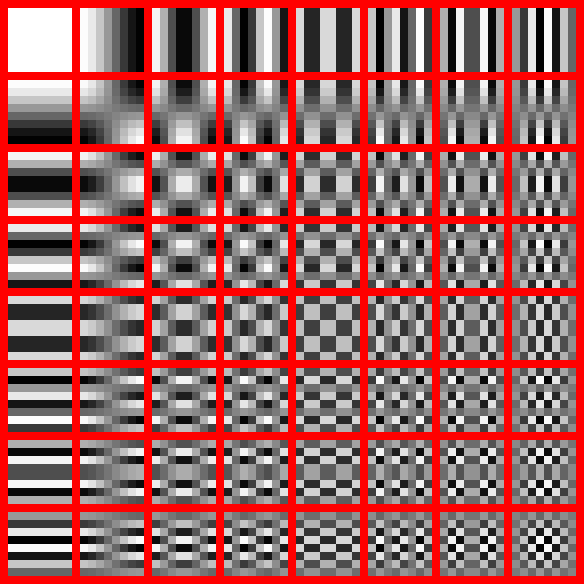
\includegraphics[width=0.5\columnwidth]{DCT.png}
	\caption{Dyskretna Transformata Kosinusowa}
\end{center}
\end{figure}
Sumując wartości pixeli z wybranych bloków, możemy uzyskać dowolną kombinację 8x8 pixeli.
\subsection{Kwantyzacja}
W kolejnym kroku następuje zmniejszenie ilości bitów potrzebnych do reprezentacji wartości pixeli.
Wartości z macierzy są dzielone przez odpowiadające wartości z tablicy kwantyzacji,
której zawartość zależy od parametru jakości przy zapisie zdjęcia (wartości są odwrotnie proporcjonalne do wartości parametru jakości).
Współczynniki w tablicy kwantyzacji rosną, zmierzając do dolnej, prawej części macierzy.
Odpowiada to zwiększaniu się zagęszczenia informacji w tablicy bloków wykorzystanej w poprzednim kroku.
Taka operacja wykorzystuje problem z rozróżnieniem informacji o dużym zagęszczeniu przez ludzkie oko.
Otrzymane wartości są zaokrąglane do najbliższej liczby całkowitej, następuje utrata danych.
\subsection{Kodowanie}
Otrzymana macierz jest spłaszczana według następującego wzorca:
\begin{figure}[h!]
	\begin{center}
	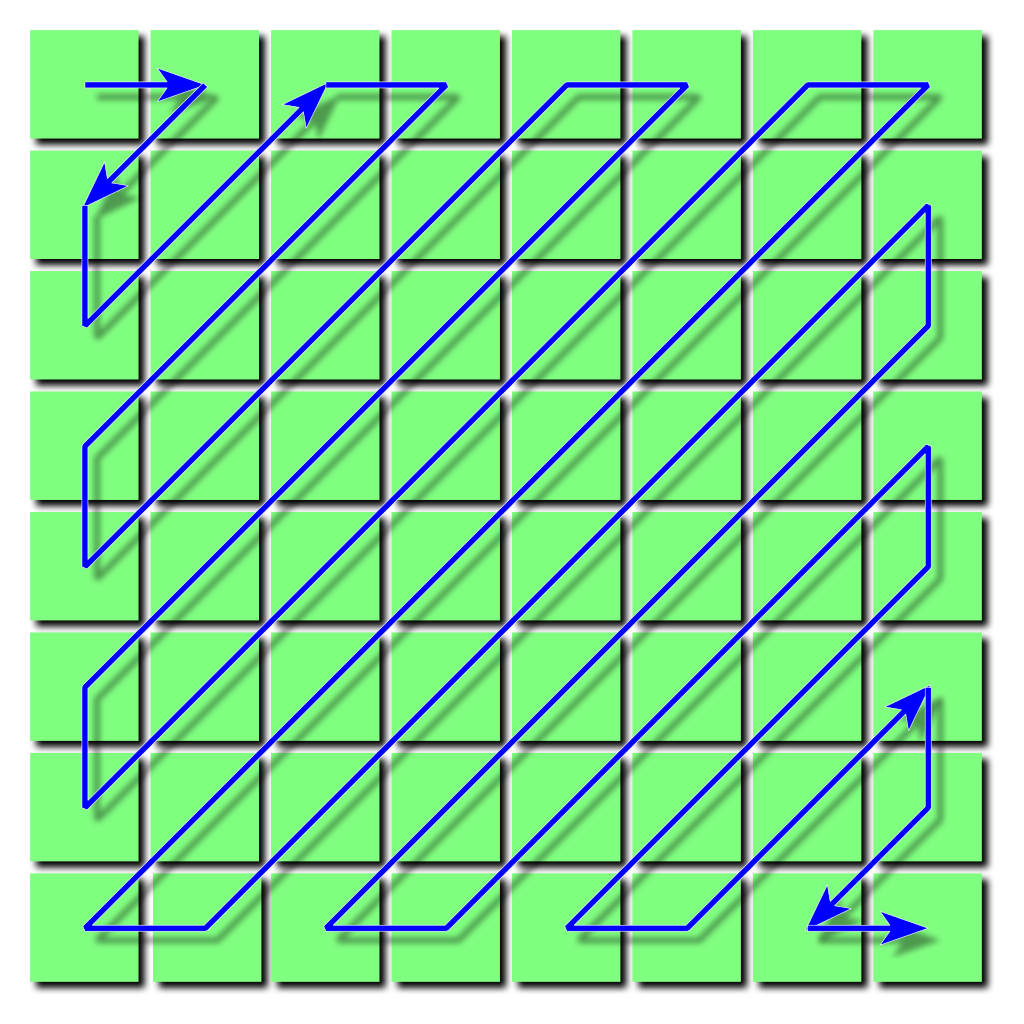
\includegraphics[width=0.5\columnwidth]{pattern.png}
	\caption{Kolejność spłaszczania segmentu}
\end{center}
\end{figure}
\\
Co zwiększa prawdopodobieństwo wystąpienia długich sekwencji zer, możliwych do zapisania w zwięźlejszy sposób.
Na koniec obraz zostaje poddany kompresji kodowaniem Huffmana.
\newpage
\section{Sieci typu U-Net}
U-Net jest architekturą sieci konwolucyjnch, najczęściej stosowaną do segmentacji obrazów. Wyróżnić można jej 2 części.
\begin{figure}[h!]
	\begin{center}
	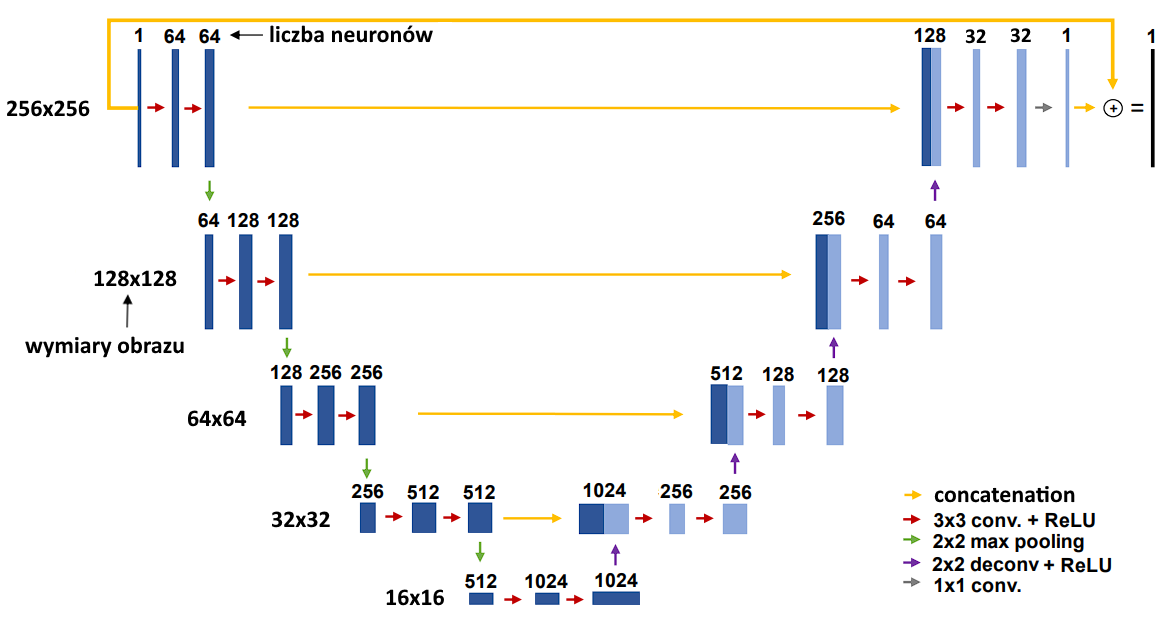
\includegraphics[width=0.9\columnwidth]{unet.png}
	\caption{Zastosowana w projekcie architektura sieci U-Net o 5 poziomach}
\end{center}
\end{figure}
\subsection{Enkoder}
Pierwszą częścią modelu jest warstwa wejściowa, w której dla każdego pixela czarno-białego obrazu wejściowego odpowiada 1 neuron.
Następnie występują 2 etapy składające się z konwolucji o jądrze 3x3 oraz funkcji aktywacji ReLu, zwiększające liczbę neuronów do 64.
Kolejnu jest powtarzalny segment składający się z Downsampling??? i konwolucji z funkcją aktywacji relu.
Skutkuje to czterokrotnym zmniejszeniem rozmiaru obrazu oraz podwojeniem liczby neuronów w każdej warstwie.
\subsection{Dekoder}
Każda z powtarzalnych warstw dekodera składa się z 3 elementów.
Pierwsza jest transponowana konwolucja o jądrze 2x2. Następnie powstała sieć jest łączona z odpowiadającą jej warstwą enkodera.
Takie połączenie przeciwdziała problemowi zanikającego gradientu - przywraca cechy wykryte w poprzednich warstwach sieci.
Po niej występują 2 warstwy konwolucji z funkcją aktywacji ReLu, takie same jak w enkoderze.
Dekoder zakończony jest spłaszczeniem obrazu do postaci, w której każdy neuron odpowiada 1 pikselowi obrazu wyjściowego.
Warstwa wyjściowa jest sumą obrazu wejściowego i spłaszczonej warstwy.
Przy takim rozwiązaniu, zwanym połączeniami rezydualnymi, sieć tworzy maskę zmian potrzebnych w obrazie wejściowym, zamiast bezpośrednio obraz przekształcać.

\section{Augmentacja danych}
Zbiór danych stanowi 16 kolorowych zdjęć wysokiej rozdzielczości, 1 czarnobiały wykres służący do kalibracji sprzętu fotograficznego,
oraz 3 wygenerowane obrazy składające się z gradientów kolorów i prostych kształtów.
Zdjęcia zostają podzielone na warstwy RGB, a następnie utworzone zostają wszystkie możliwe kombinacje obróceń i odbić obrazu.
Następuje pocięcie zdjęć na kwadratowe segmenty o zadanym rozmiarze.
Oryginał segemntu zostaje zapisany przy ustawieniu jakości równym 100 wykorzystywana jako maska w modelu.
Dane uczące zostaja zapisane przy ustawieniu równym 25, przy którym artefakty kompresji zaczynają być łatwo zauważalne.
W przypadku podziału na segmenty o rozmiarze 256x256 pixeli otrzymujemy 9500 próbek w zbiorze testowym, oraz 1000 w zbiorze walidacyjnym.

\section{Model i szkolenie}
Podstawową architekturą w projekcie jest, najczęściej stosowana, sieć o 5 poziomach.
Podczas uczenia utworzone zostają generatory danych testowych i walidacyjnych.
Zawierają one skompresowane oraz oryginalne obrazy, te drugie wykorzystywane w modelu jako maska.
Pogrupowane zostają w paczki po 3.
Podczas jednego kroku uczenia, wykorzystane zostaje, losowo wybrane, 10\% paczek ze zbioru uczącego.
Proces uczenia trwa 100 epok.
Dane uczące i walidacyjne wybierane są na podstawie stałego ziarna, co pozwala na porównanie wyników modeli.
Jako funkcję straty wybrana została wartość bezwzględna błędu, optimizer??? to Adam o współczynniku uczenia 0.0001.

\begin{figure}[h!]
\begin{center}
	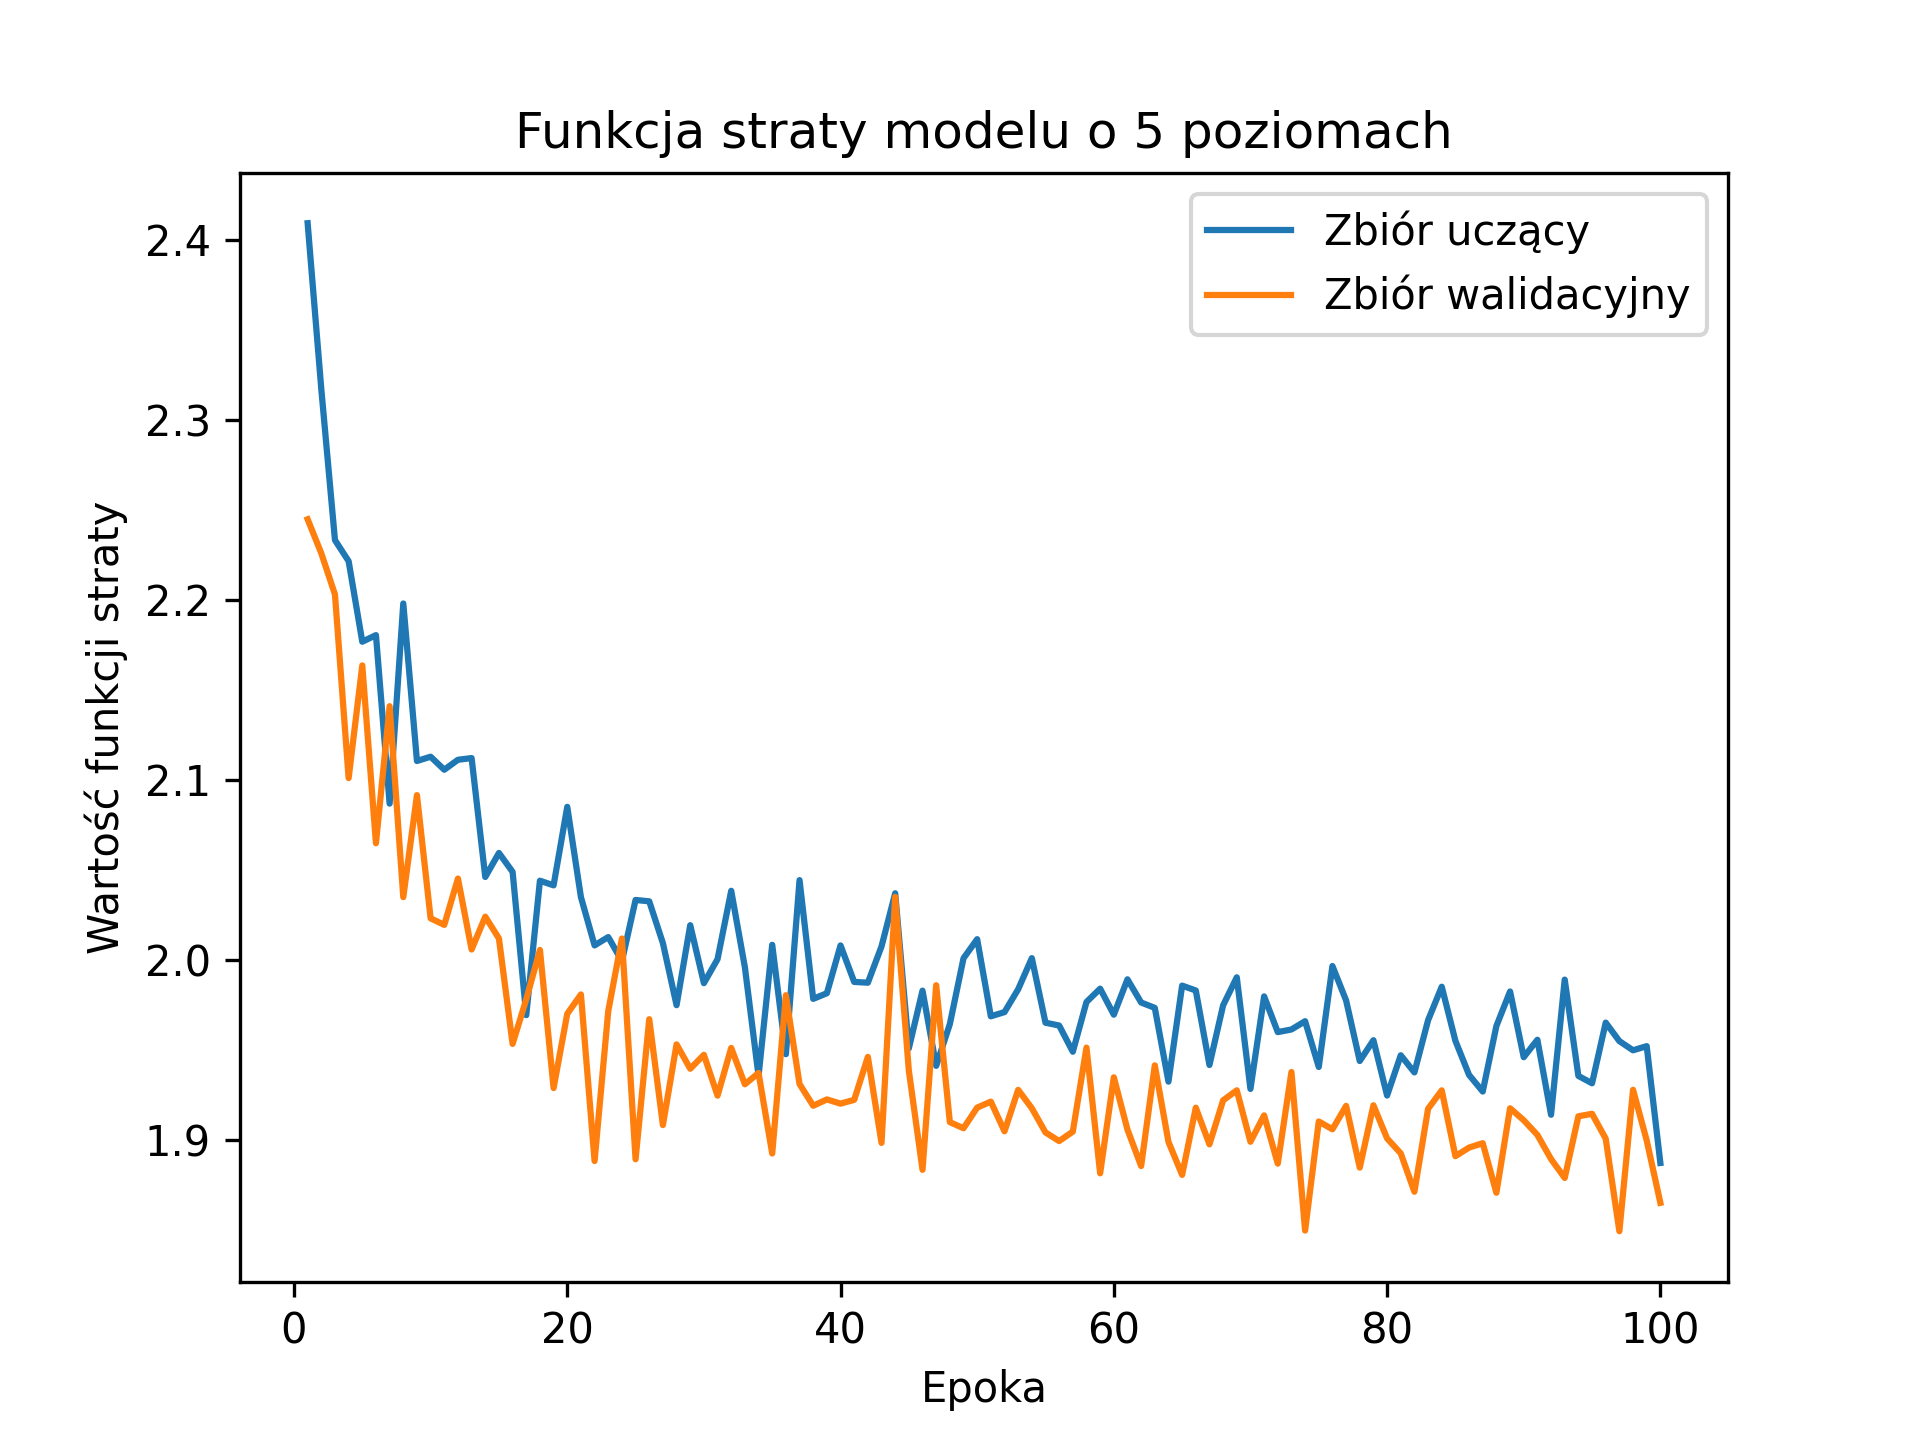
\includegraphics[width=0.7\columnwidth]{loss5.png}
	\caption{Funkcja straty}
\end{center}
\end{figure}

Zauważyć można, że po 20 epoce, tempo zmniejszania wartości funkcji straty znacząco maleje,
a po 60 epoce praktycznie zatrzymuje.
Wartym uwagi jest niższa wartość straty w zbiorze walidacyjnym niż uczącym. Jako, że zbiory zostały utworzone z tych samych zdjęć,
prawdopodobnie jest, że to losowy przypadek w wybranym ziarnie generatora danych.
Podczas uczenia dokładność była znikoma i stała. Nie jest ona jednak miarodajną metryką, gdyż oczekuje dokładnych wartości pixeli.
Człowiek nie jest w stanie rozpoznać małych różnić w wartościach RGB, w związku z czym ważna była jedynie wartość funkcji straty.

\section{Wyniki działania modelu}
W sekcji przedstawione zostały wyniki działania odtwarzania obrazów modelem o 5 warstwach,
rozmiarze segmentu 256x256 oraz 8 pixelach przesunięcia przy odtawarzaniu (proces opisany w sekcji 8).
\newpage
\subsection{Roślinność na tle kamiennej ściany}
\begin{figure}[h!]
\begin{center}
	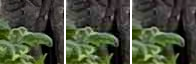
\includegraphics[width=0.85\columnwidth]{compare_sample.png}
	\caption{Zestawienie obrazów oryginalnego, skompresowanego, oraz odtworzonego przez sieć}
\end{center}
\end{figure}
\begin{figure}[h!]
\begin{center}
	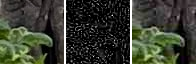
\includegraphics[width=0.85\columnwidth]{orig_vs_comp.png}
	\caption{Różnice między obrazem oryginalnym i skompresowanym}
\end{center}
\end{figure}
\begin{figure}[h!]
\begin{center}
	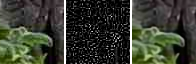
\includegraphics[width=0.85\columnwidth]{comp_vs_rest.png}
	\caption{Różnice między obrazem skompresowanym i odtworzonym}
\end{center}
\end{figure}
\begin{figure}[h!]
\begin{center}
	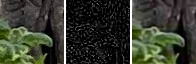
\includegraphics[width=0.85\columnwidth]{orig_vs_rest.png}
	\caption{Różnice między obrazem oryginalnym i odtworzonym}
\end{center}
\end{figure}

\newpage
\subsection{Zarost na twarzy}
\begin{figure}[h!]
\begin{center}
	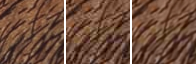
\includegraphics[width=0.85\columnwidth]{compare_sample2.png}
	\caption{Zestawienie obrazów oryginalnego, skompresowanego, oraz odtworzonego przez sieć}
\end{center}
\end{figure}
\begin{figure}[h!]
\begin{center}
	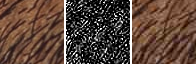
\includegraphics[width=0.85\columnwidth]{orig_vs_comp2.png}
	\caption{Różnice między obrazem oryginalnym i skompresowanym}
\end{center}
\end{figure}
\begin{figure}[h!]
\begin{center}
	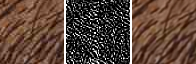
\includegraphics[width=0.85\columnwidth]{comp_vs_rest2.png}
	\caption{Różnice między obrazem skompresowanym i odtworzonym}
\end{center}
\end{figure}
\begin{figure}[h!]
\begin{center}
	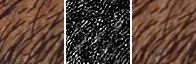
\includegraphics[width=0.85\columnwidth]{orig_vs_rest2.png}
	\caption{Różnice między obrazem oryginalnym i odtworzonym}
\end{center}
\end{figure}
\subsection{Spostrzeżenia}
Zauważalna jest utrata detali względem obrazu oryginalnego, a nawet względem obrazu skompresowanego. Sieć ma cechy filtra uśredniającego.
W porównaniach widoczna jest siatka kwadratów o boku 8 pixeli, wynikajaca ze sposobu działania algorytmu JPEG.
Różnica między obrazem oryginalnym i odtworzonym jest mniejsza niż między obrazem oryginalnym i skompresowanym oraz skompresowanym i odtworzonym.

\section{Wybór optymalnej architektury}
Ważnym przy wyborze architektury sieci jest jej złożoność, nadmierna negatywnie wpływa na czas uczenia pomimo znikomej poprawy wartości funkcji błędu.
\subsection{Liczba poziomów sieci}
Przetestowane zostały sieci od 1 do 5 poziomów. Każda została wyszkolona w takich samych warunkach i przy stałym ziarnie generatora danych.
\begin{figure}[h!]
\begin{center}
	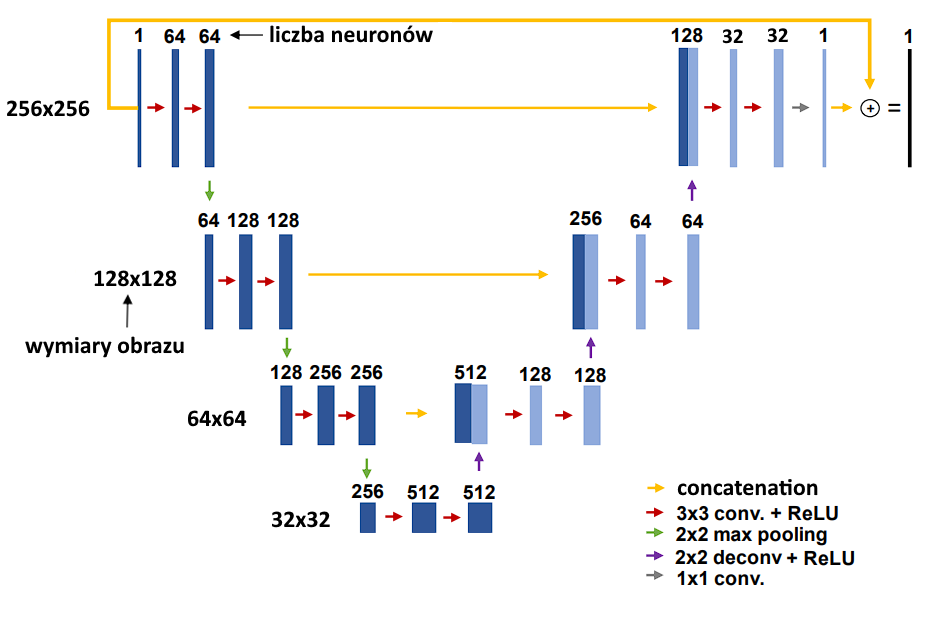
\includegraphics[width=0.9\columnwidth]{unet4.png}
	\caption{Architektura sieci U-Net o 4 poziomach}
\end{center}
\end{figure}
\newpage
\subsection{Spostrzeżenia}
\begin{figure}[h!]
\begin{center}
	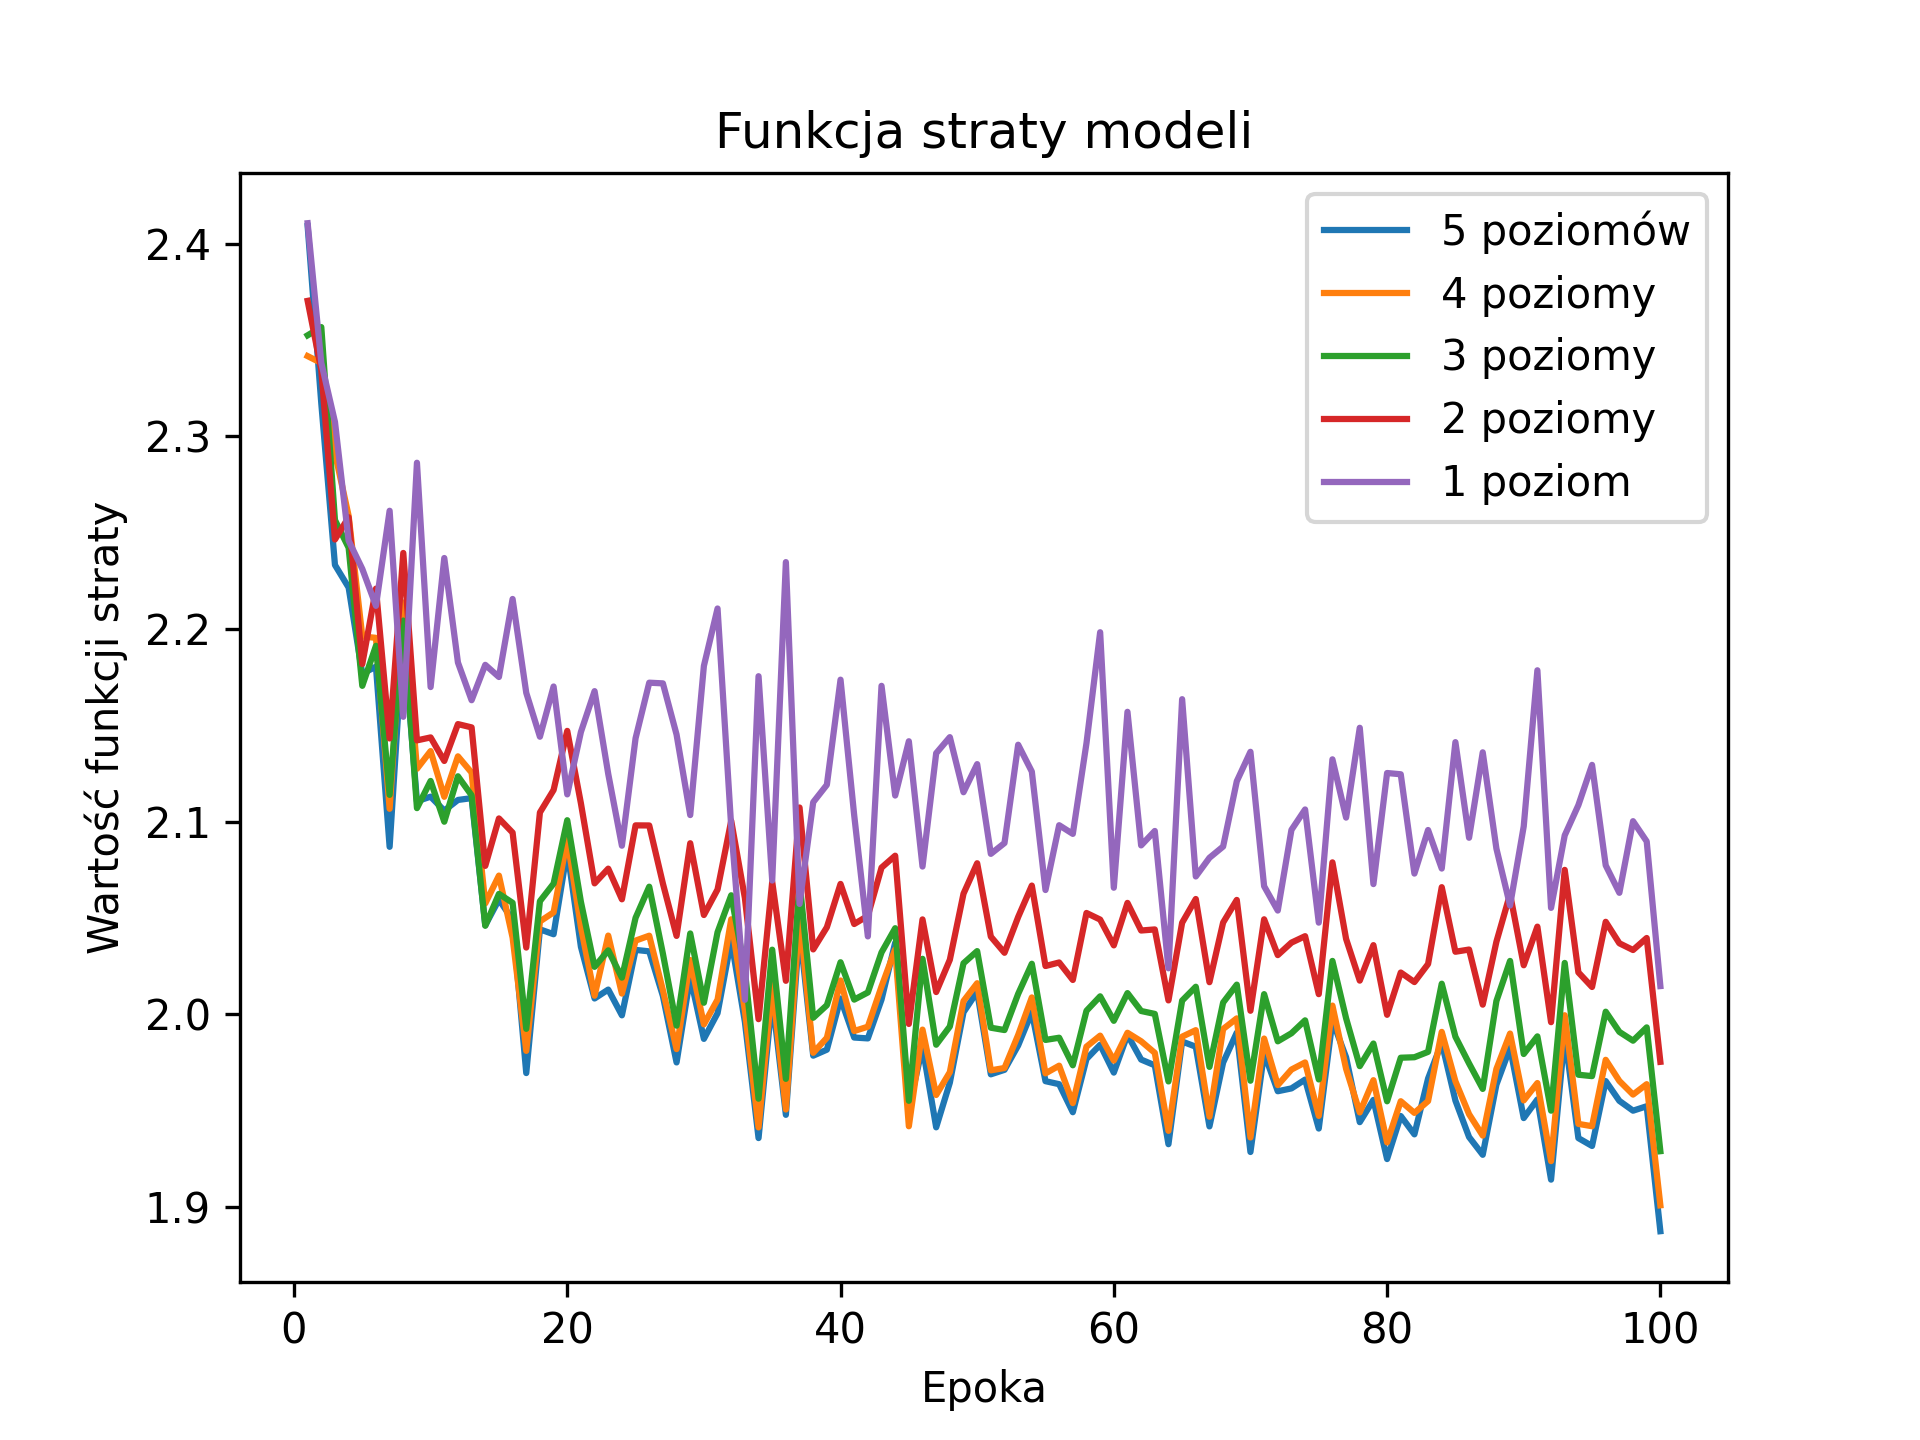
\includegraphics[width=0.7\columnwidth]{layers.png}
	\caption{Funkcja straty przy różnej liczbie poziomów sieci}
\end{center}
\end{figure}
Zauważyć można zbliżone wyniki sieci o 3, 4 i 5 poziomach.
Dla 1 i 2 poziomów wystąpiło znaczące pogorszenie wyników. Zmiana wartości funkcji straty spowolniła przy podobnej liczbie epok.
Wynika z tego, że do problemu wystarczy zastosowania sieci o 3 lub 4 poziomach, co przyśpieszy proces uczenia.
\subsection{Rozmiar obrazu wejściowego}
Przetestowany został również wpływ rozmiaru obrazu wejściowego na wartość funkcji straty, przy 5 poziomach sieci.
\\
\begin{figure}[h!]
\begin{center}
	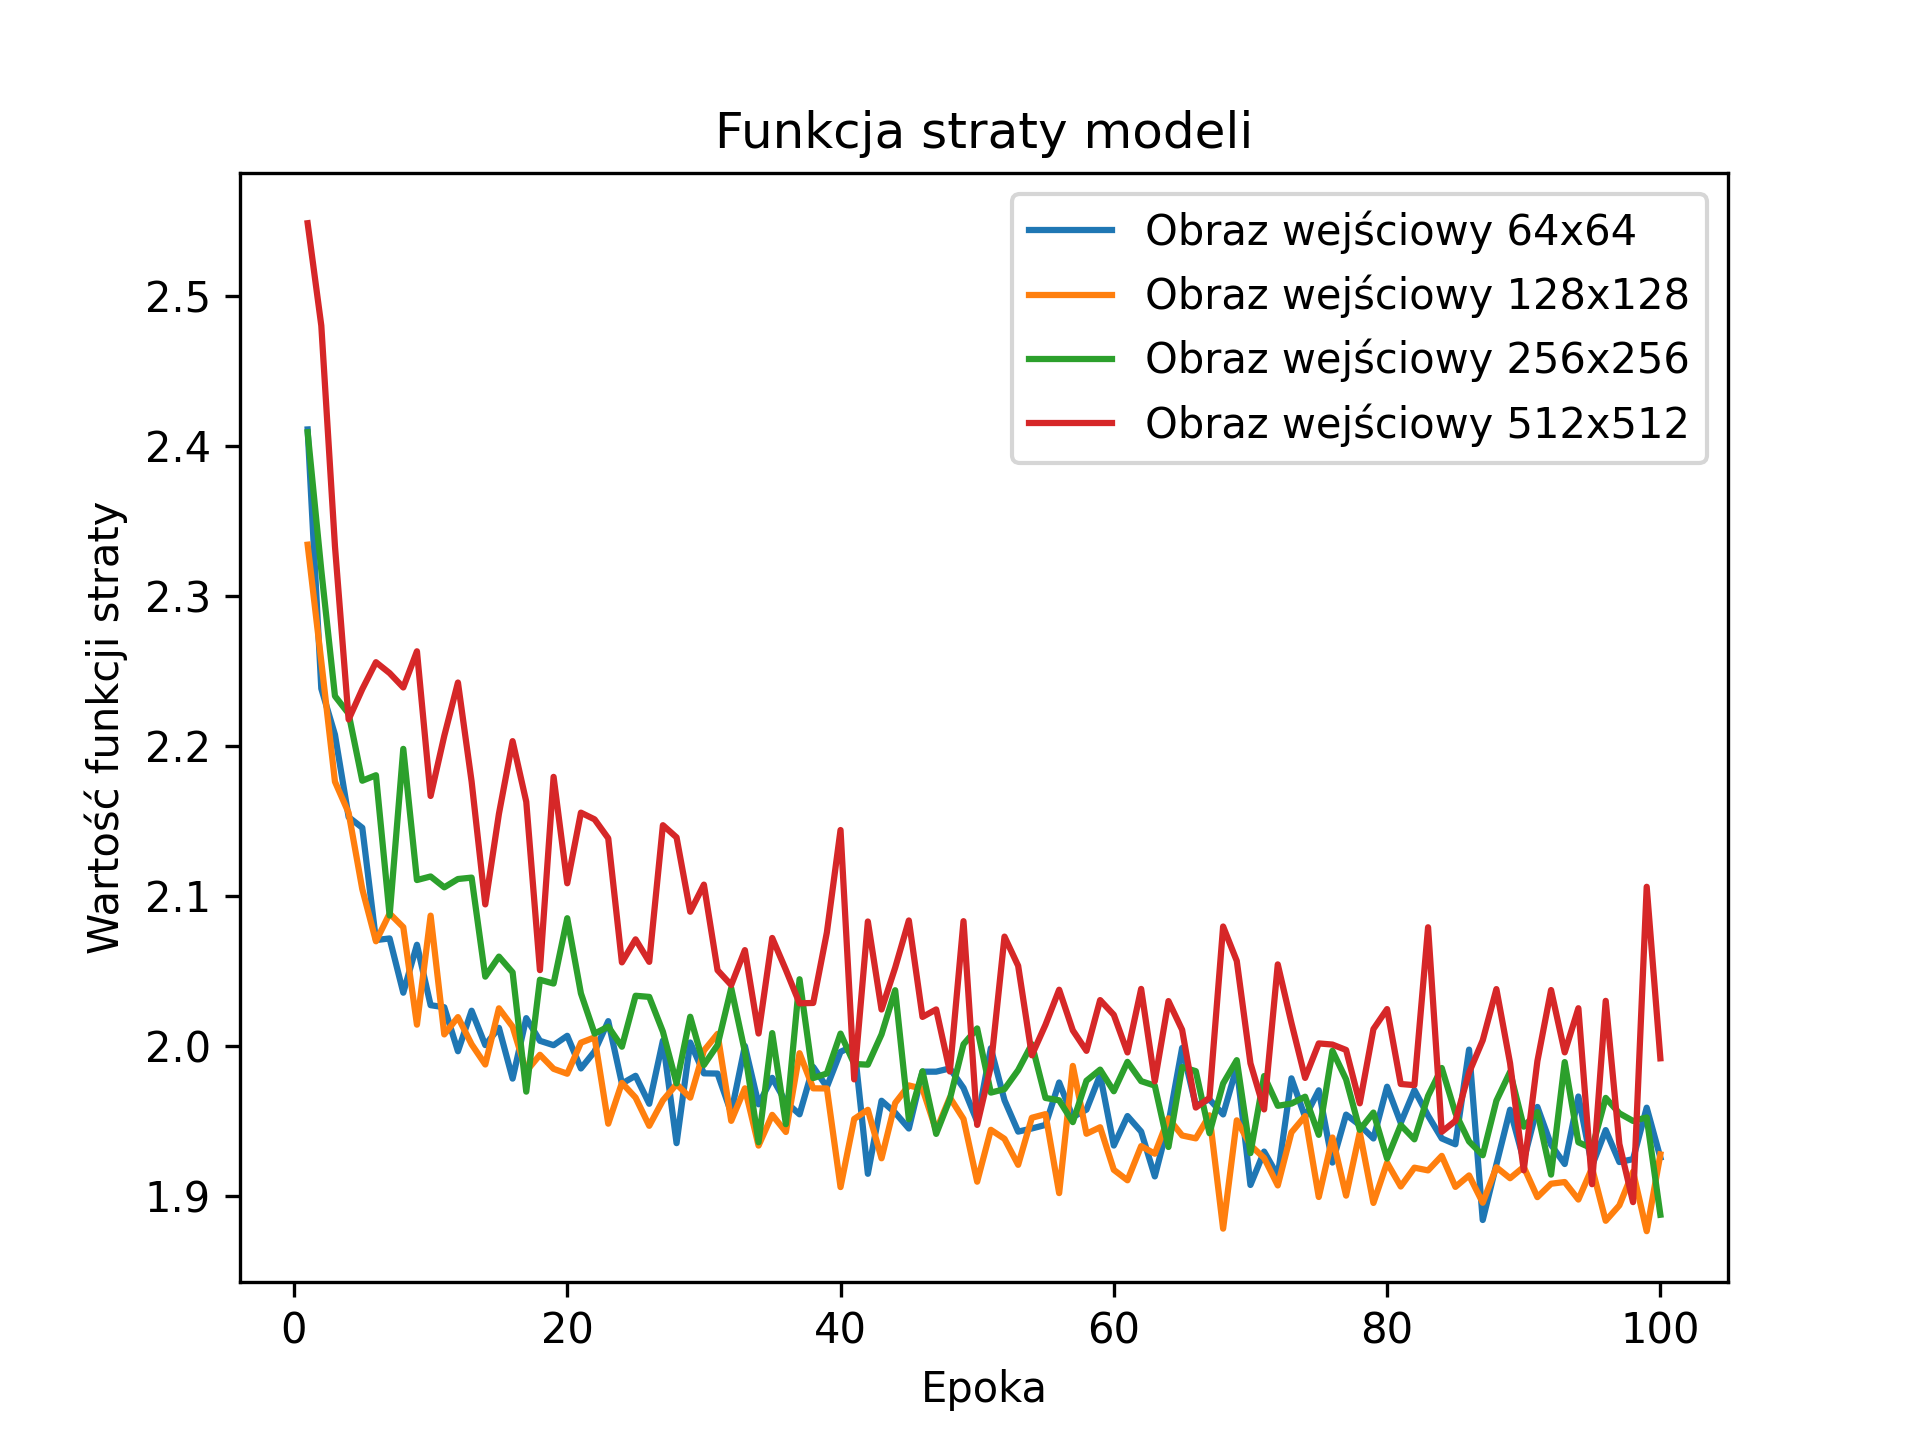
\includegraphics[width=0.7\columnwidth]{size.png}
	\caption{Funcja straty przy różnych rozmiarach obrazu wejściowego}
\end{center}
\end{figure}
Zauważyć można podobne wyniki dla obrazów o rozmiarze 64x64 oraz 128x128 pixeli.
Dla obrazu o rozmiarach 128x128 pixeli zauważyć można nieznacznie lepsze wyniki dla końcowych epok.
Jest to jednak skutkiem przetrenowania, gdyż wartość funkcji straty w zbiorze walidacyjnym pozostawała stała.
W przypadku obrazu o rozmiarze 512x512 pixeli nastąpiło znaczące pogorszenie wyników.
Zasugerować można wybór dowolnego z rozmiarów 64x64, 128x128 oraz 256x256 pixeli.
Należy jednak pamiętać, że mniejszy rozmiar obrazu wejściowego, choć przyśpiesza szkolenie,
proporcjonalnie wpływa na czas odtwarzania pełnego obrazu.

\section{Oddtwarzanie pełnego obrazu}
Sieć została przystosowana do przetwarzania jednowymiarowych obrazów o rozmiarze 256x256 pixeli.
Tworzy to potrzebę przystosowania rozwiązania do przetwarzania obrazów o dowolnym rozmiarze.
Obraz zostaje podzielony na kanały RGB, a następnie, kolejne segmenty każdej warstwy są przetwarzane przez model.
Wartości otrzymanej macierzy są zaokrąglane do liczb całkowitych oraz następuje winsoryzacja wartości spoza zakresu 0-255.
W przypadku segmentów na krawędziach obrazu, brakujący fragment zostaje uzupełniony lustrzanym odbiciem obrazu a po szkoleniu odcięty.
Z podejściem wiąże się problem, widocznych granic między przetworzonymi segmentami.
Rozwiązaniem jest częściowe pokrycie segmentów przy przetwarzaniu oraz zastosowanie średniej ważonej na ich granicy.

\begin{figure}[h!]
\begin{center}
	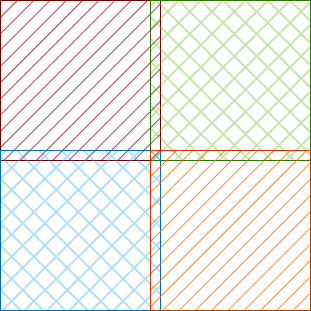
\includegraphics[width=0.5\columnwidth]{overlap.png}
	\caption{Nachodzace na siebie segmenty obrazu}
\end{center}
\end{figure}

Pomimo zastosowania średniej ważonej, na granicy segmentów często pozostaje widoczna linnia.
Problem ten można rozwiązać poprzez wybranie odpowiedniej wartości przesunięcia segmentów.
\begin{figure}[h!]
\begin{center}
	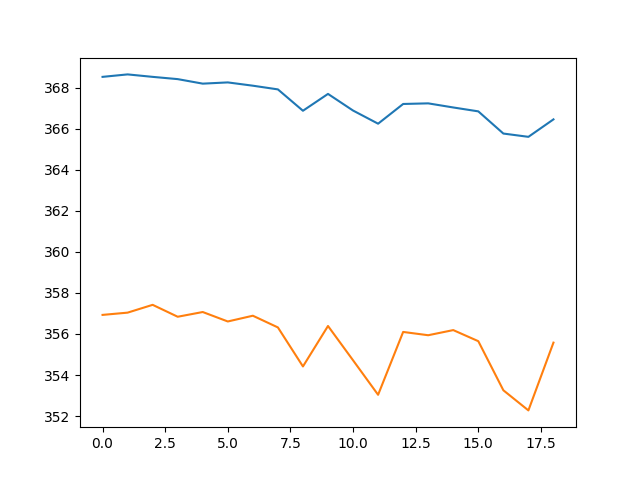
\includegraphics[width=0.7\columnwidth]{overlap_and_loss.png}
	\caption{Wartość funkcji błędu dla różnych wartości przesunięcia}
\end{center}
\end{figure}
Zauważyć można spadek wartości dla przesunięcia o 8 i 16 pixeli. Jest to związane z podziałem obrazu na obszary 8x8 przez algorytm JPEG.
Jeżeli krawędzie powstałe w wyniku przetwarzania obrazu pokryją się z krawędziami powstającymi przy kompresji,
wynikowy błąd będzie mniejszy niż w przypadku, gdyby na obrazie tworzyły się dodatkowe granice.
Dodatkowo widoczny jest spadek dla 11 pixeli, dla którego nie znam wyjaśnienia.
Wartość 8 pixeli została wybrana jako optymalna, przy większych wartościach pojawia się ryzyko rozmazania obrazu przez średnią ważoną.


\section{Sieci konwolucyjne}
\section{Wnioski}
Można zastosować sieci typu U-Net do usuwania artefaktów kompresji stratnej.
Takie rozwiązanie jest jednak bardzo wolne. Przetworzenie obrazu o wymiarach 3024x4032 pixeli zajmuje około 80 sekund.
Optymalne wydaje się zastosowanie sieci o 4 poziomach, przy rozmiarze obrazu wejściowego 256x256 pixeli.
Przy odtwarzaniu obrazu należy zastosować przesunięcie 8 pixeli, aby granice między segmentami pokryły się z granicami powstałymi w wyniku działania algorytmu JPEG.

\section{Źródła}
\begin{itemize}
\item https://cgjennings.ca/articles/jpeg-compression/
\item U-Net: Convolutional Networks for Biomedical Image Segmentation [Olaf Ronneberger, Philipp Fischer, Thomas Brox]
\item 3D U-Net: Learning Dense Volumetric Segmentation from Sparse Annotation [Özgün Çiçek,Ahmed Abdulkadir, Soeren S. Lienkamp, Thomas Brox, Olaf Ronneberger]
\item Deep Learning for Photoacoustic Tomography from Sparse Data [Stephan Antholzer, Markus Haltmeier, Johannes Schwab]
\item Fully Dense UNet for 2D Sparse Photoacoustic Tomography Artifact Removal [Steven Guan, Amir A. Khan, Siddhartha Sikdar, Parag V. Chitnis]
\item Deep Residual Learning for Image Recognition [Kaiming He, Xiangyu Zhang, Shaoqing Ren, Jian Sun]

\end{itemize}
\end{document}
